\newpage
\section{Задание 3.}

Найти объем тела, ограниченного данными поверхностями, с помощью тройного интеграла.

$$x = 2y^2 + 3, x = 5, z = 1 + \sqrt{9x^2 + 4y^2}, z = 4 + \sqrt{9x^2 + 4y^2}$$

Попробуем найти границы интегрирования. Чтобы $x$ был ограничен, нужно, чтобы уравнение $x=5$ было его верхней границей. Тогда нижней границей станет $2y^2+3$. Отсюда можно найти, как меняется $y$. 

$$2y^2 + 3 < 5 \Rightarrow 2y^2 < 2 \Rightarrow y^2 < 1 \Rightarrow y\in(-1,1)$$

Для $z$ просто возьмем уравнения из условия, так как $x$ и $y$ уже найдены. Теперь можно записать интеграл объема.
$$V = \int_{-1}^{1}\,  dy. \int_{2y^2+3}^{5} dx \,\int_{1+\sqrt{9x^2+4y^2}}^{4+\sqrt{9x^2+4y^2}} \, dz $$
\begin{center}
Интегрируем по $z$.
$$ \int_{1+\sqrt{9x^2+4y^2}}^{4+\sqrt{9x^2+4y^2}} dz = [z]_{1+\sqrt{9x^2+4y^2}}^{4+\sqrt{9x^2+4y^2}} = (4+\sqrt{9x^2+4y^2}) - (1+\sqrt{9x^2+4y^2}) = 3.$$
Тогда интеграл объема можно упростить.
$$V = \int_{-1}^{1}\,  dy. \int_{2y^2+3}^{5} \,dx \int_{1+\sqrt{9x^2+4y^2}}^{4+\sqrt{9x^2+4y^2}} \, dz  = \int_{-1}^{1}\,  dy. \int_{2y^2+3}^{5} 3 \,dx $$
Интегрируем по $x$.
$$\int_{2y^2+3}^{5} 3 \, dx = 3 \left[ x \right]_{2y^2+3}^{5} = 3 \left( 5 - (2y^2 + 3) \right) = 3(2 - 2y^2) = 6(1 - y^2) \Rightarrow$$
$$\Rightarrow V = \int_{-1}^{1}\,  dy. \int_{2y^2+3}^{5} 3 \,dx = \int_{-1}^{1} 6(1 - y^2) \,dy. $$
Интегрируем по $y$.
$$V = \int_{-1}^{1} 6(1-y^2) \, dy = 6 \int_{-1}^{1} (1-y^2) \, dy = 6 \left[ y - \frac{y^3}{3} \right]_{-1}^{1} = 6 \left( \left(1 - \frac{1}{3}\right) - \left(-1 + \frac{1}{3}\right) \right) = 6 \left( \frac{2}{3} + \frac{2}{3}\right) = \boxed{8}$$
\end{center}

% \vspace{2em}

% \href{https://www.desmos.com/3D/wpt0hvgifd}{Посмотреть фигуру в 3D}\quad
% \href{https://www.desmos.com/3D/wpt0hvgifd}{Посмотреть сечение $XZ$ в $y=0$}
\begin{figure}[h!t]
    \centering
    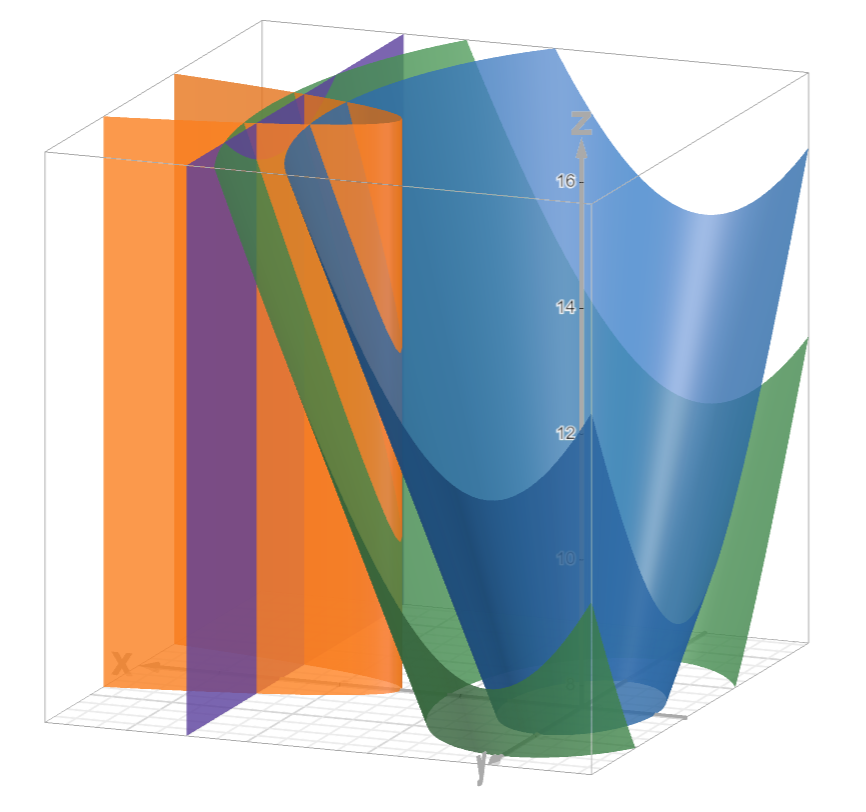
\includegraphics[width=0.4\linewidth]{Task3/Figure_outer_shapes.png}
    \caption{Задание 3. Ограничивающие поверхности \underline{\href{https://www.desmos.com/3D/kl5guofsih}{(Desmos)}}. }
\end{figure}
\newpage

\begin{figure}[h!t]
    \centering
    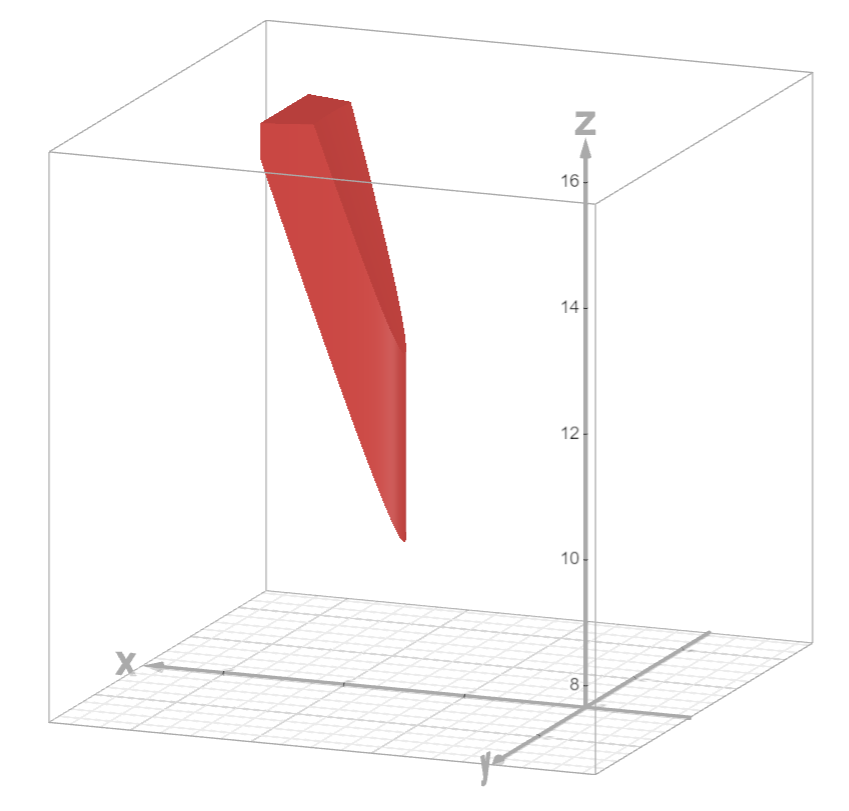
\includegraphics[width=0.6\linewidth]{Task3/Figure_volume_shape.png}
    \caption{Задание 3. Тело, которое задано поверхностями \underline{\href{https://www.desmos.com/3D/kl5guofsih}{(Desmos)}}. }
\end{figure}

\begin{figure}[h!t]
    \centering
    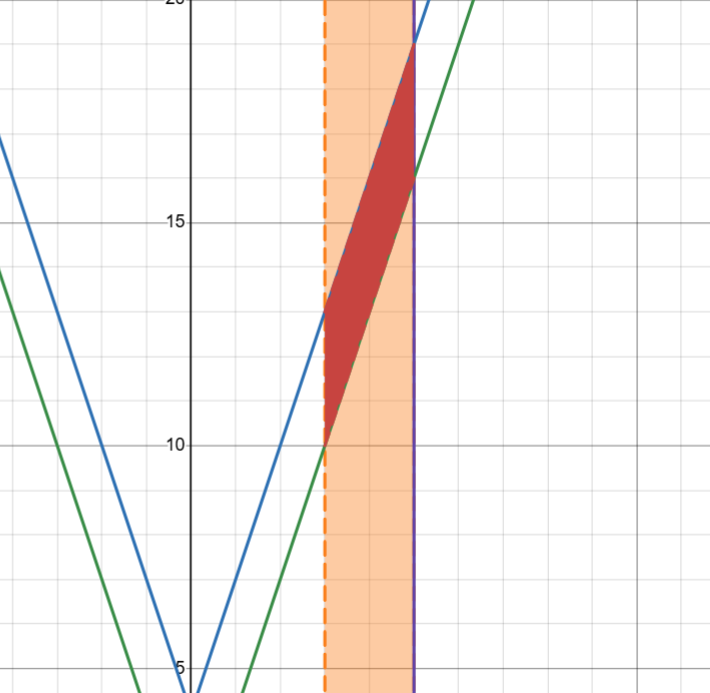
\includegraphics[width=0.6\linewidth]{Task3/Figure_XZ_intersection.png}
    \caption{Задание 3. Сечение по плоскости $XZ$ при $y=0$ \underline{\href{https://www.desmos.com/Calculator/q5wb8deh0a}{(Desmos)}}. }
\end{figure}
